\section{Defination}

Vài cái định nghĩa cơ bản, thêm sau

\begin{theorem}[Euler's formula]
    $V-E+F=2$ for convex polyhedra
\end{theorem}
But we will generalize it to planar graphs by using stereographic projection

First, we see that we can take a graph embedded on the surface of a sphere and under stereographic projection get a planar graph \\

\begin{figure}[H]

    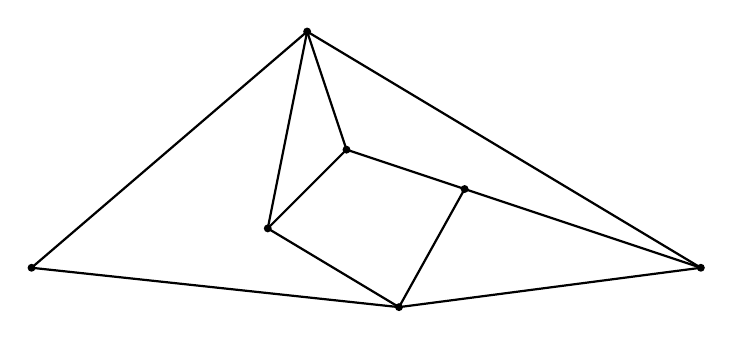
\begin{tikzpicture}[scale = 0.5]
        \draw[black, thick] (-7,-1) -- (7/3,-2);
        \draw[black, thick] (-7,-1) -- (0,5);
        \draw[black, thick] (-1,0) -- (7/3,-2);
        \draw[black, thick] (-1,0) -- (0,5);
        \draw[black, thick] (-1,0) -- (1,2);
        \draw[black, thick] (10,-1) -- (1,2);
        \draw[black, thick] (0,5) -- (1,2);
        \draw[black, thick] (0,5) -- (10,-1);
        \draw[black, thick] (4,1) -- (7/3,-2);
        \draw[black, thick] (10,-1) -- (7/3,-2);

        \filldraw[black, thick] (-1,0) circle (2pt);
        \filldraw[black, thick] (4,1) circle (2pt);
        \filldraw[black, thick] (10,-1) circle (2pt);
        \filldraw[black, thick] (-7,-1) circle (2pt);
        \filldraw[black, thick] (1,2) circle (2pt);
        \filldraw[black, thick] (0,5) circle (2pt);
        \filldraw[black, thick] (7/3,-2) circle (2pt);
    \end{tikzpicture}
\end{figure}

\begin{figure}[H]

    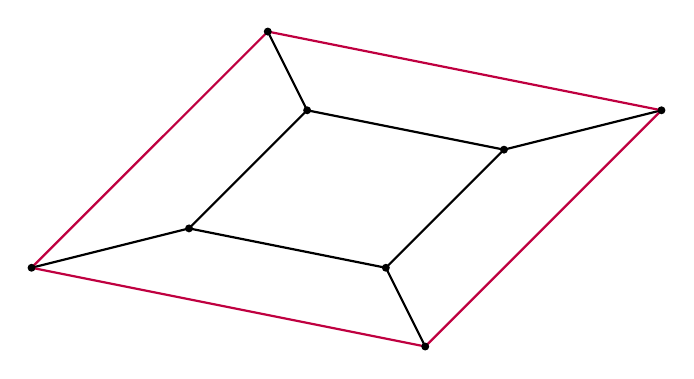
\begin{tikzpicture}[scale = 0.5]
        \draw[black, thick] (-1,2) -- (-2,4);
        \draw[black, thick] (-4,-1) -- (-8,-2);
        \draw[black, thick] (4,1) -- (8,2);
        \draw[black, thick] (1,-2) -- (2,-4);
        \draw[black, thick] (-1,2) -- (-4,-1);
        \draw[black, thick] (-4,-1) -- (1,-2);
        \draw[black, thick] (1,-2) -- (4,1);
        \draw[black, thick] (4,1) -- (-1,2);
        \draw[purple, thick] (-2,4) -- (-8,-2);
        \draw[purple, thick] (-8,-2) -- (2,-4);
        \draw[purple, thick] (2,-4) -- (8,2);
        \draw[purple, thick] (8,2) -- (-2,4);

        \filldraw[black, thick] (-1,2) circle (2pt);
        \filldraw[black, thick] (-2,4) circle (2pt);
        \filldraw[black, thick] (-4,-1) circle (2pt);
        \filldraw[black, thick] (-8,-2) circle (2pt);
        \filldraw[black, thick] (4,1) circle (2pt);
        \filldraw[black, thick] (8,2) circle (2pt);
        \filldraw[black, thick] (1,-2) circle (2pt);
        \filldraw[black, thick] (2,-4) circle (2pt);
    \end{tikzpicture}
\end{figure}
